\begin{figure*}[t]
  \centering
  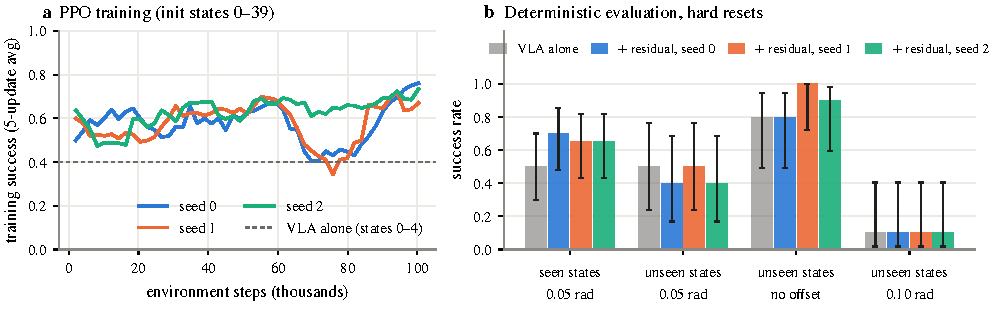
\includegraphics[width=\textwidth]{figures/rl_residual.pdf}
  \caption{\textbf{Residual RL on the arm-offset weakness} (LIBERO-Spatial task 2, offset 0.05\,rad per
  joint). (a)~Success of the stochastic policy during PPO, moving average over 5 updates (about 60
  episodes). (b)~Deterministic evaluation with hard resets, on initial states seen during training
  (0--19, 20 episodes) and on held-out ones (40--49, 10 episodes per bar). Wilson 95\% intervals.}
  \label{fig:rl}
\end{figure*}

\subsection{A residual corrector learns, but does not generalise}
\textbf{Target and design.} The arm-offset weakness is a natural target: the perturbation is visible in
proprioception, so a corrector without images can in principle detect it. We use LIBERO-Spatial task 2
at 0.05\,rad per joint, where the VLA alone succeeds in about half of the episodes. The corrector is an MLP
(two hidden layers of 128) that sees end-effector position and orientation, gripper opening, the VLA's
proposed action and the episode progress, and outputs $\Delta a\in[-1,1]^7$; the executed action is
$\mathrm{clip}(a_{\mathrm{VLA}} + 0.2\,\Delta a)$. Its last layer is initialised to zero, so before
training it reproduces the VLA exactly; we checked this on full episodes (identical outcomes and episode
lengths). It is trained with PPO~\citep{schulman2017ppo} in a single-file implementation in the style of
CleanRL~\citep{huang2022cleanrl}, with a sparse reward (1 on success), $\gamma=0.995$, four simulators in
one process sharing batched VLA calls, and 100k environment steps per run (about 400 episodes, 3\,h on
the laptop at 10 steps/s). Training uses initial states 0--39; states 40--49 are kept for evaluation.

\textbf{Results} (Fig.~\ref{fig:rl}). Training success rises modestly (from \RLTrainFirst{} to
\RLTrainLast{} over the first and last ten updates of each of the \RLSeeds{} seeds); seeds 0 and 1 dip around 70k steps before recovering, seed 2 does not. On initial states seen in training, the deterministic corrector succeeds in
\RLSeenRes{} episodes against \RLSeenVla{} for the VLA alone, and every discordant episode favours the
corrector (McNemar $p=$ \RLPSeen{}, not significant at this sample size). On held-out initial states the
gain disappears: \RLUnseenRes{} against \RLUnseenVla{} at the training level, \RLUnseenStrongRes{} against
\RLUnseenStrongVla{} at 0.10\,rad, and \RLUnseenCleanRes{} against \RLUnseenCleanVla{} without offset
(so the corrector does not hurt the unperturbed task).

What does transfer is speed: successful episodes are shorter with the corrector, from \RLStepsSeenVla{} to
\RLStepsSeenRes{} steps on seen states and from \RLStepsUnseenVla{} to \RLStepsUnseenRes{} on held-out
ones. This is what the objective rewards most directly: with discounting a faster success is worth more,
and speeding up an episode that already works is observed in every rollout, whereas recovering a failure
is a rare event in 400 episodes. The recoveries that do happen are tied to the configurations seen in
training; with 40 of them, the corrector has little to interpolate from.

Drawing new offset signs at every training reset, to expose the corrector to more varied starting poses,
gives the same pattern (\RLRandSeenRes{} on seen and \RLRandUnseenRes{} on held-out initial states), so the
variety of arm offsets is not what limits generalisation.

A training-free alternative, executing 10 instead of 50 actions per chunk so that the VLA re-plans five
times more often, gives \RLReplanClean{}, \RLReplanTrain{} and \RLReplanStrong{} on the same held-out
episodes (no offset, 0.05 and 0.10\,rad), not distinguishable from the VLA alone with 10 episodes, at
\RLReplanSlowdown{}$\times$ the cost.
